
\documentclass{beamer}
\usetheme{Madrid}

\newcommand{\blue}[1]{\textcolor[rgb]{.15,0,.85}{\textbf{#1}}}
\newcommand{\red}[1]{\textcolor[rgb]{.8,0,.2}{#1}}

\title{The Lorenz Model}
\subtitle{Final Project Presentation}
\author{\textbf{Phil Mayer}}
\institute{Fairfield University}
\date[Final Presentation]{PS215 Computational Physics \\ May 5, 2016}

\begin{document}

\frame{\titlepage}

\frame{
	\frametitle{Introduction}
	
	\begin{columns}
		\column{0.6\textwidth}
		\begin{itemize}
			\item{For my final project, I chose to study the \blue{Lorenz model} (also known as the Lorenz equations), a system of nonlinear
			differential equations.}
			\item{Originally studied by Edward Norton Lorenz while trying to numerically solve the Navier-Stokes equations.}
			\item{Oversimplified the Navier-Stokes equations considerably, but discovered a system with rich dynamics and chaotic behavior.}
		\end{itemize}
		
		\column{0.02\textwidth}
		
		\column{0.38\textwidth}
		\begin{figure}
			\centering
			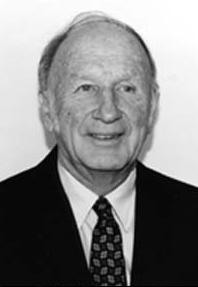
\includegraphics[scale=0.40]{elorenz.jpg}
			\caption{E.N. Lorenz, a pioneer in the study of chaos and a meteorologist. Image: Wikimedia Commons.}
		\end{figure}
	\end{columns}
}

\frame{
	\frametitle{Introduction (continued)}
	
	\begin{columns}
		\column{0.6\textwidth}
		\begin{itemize}
			\item{The Lorenz model consists of three equations, given on the right.}
			\item{Though often given physical meaning, the model itself is mathematical. We might picture the (deterministic) motion of a particle
			in three dimensions. }
			\item{Uses three parameters: $\sigma$, $r$, and $b$, each positive. }
			\item{By convention, we typically choose $\sigma = 10$ and $b = \frac{8}{3} \approx 2.6667$.}
		\end{itemize}

		\column{0.40\textwidth}
		\begin{align*}
			\frac{dx}{dt} &= \sigma(y - x) \\
			\frac{dy}{dt} &= -xz + rx - y \\
			\frac{dz}{dt} &= xy - bz
		\end{align*}
	\end{columns}
}

\frame{
	\frametitle{Numerical Methods}
	
	\begin{itemize}
		\item{Since we have three first-order ODEs, the obvious solution is to employ the Euler method.}
		\item{As we will see shortly, many of the solution graphs exhibit oscillatory behavior. While the Euler-Cromer method tends to be more 
		stable for oscillatory problems, the parameters minimize the error (given high precision).}
		\item{Recall that the Euler method is easy to derive:
		Given $n$ points indexed as $x_i$ (over $1 \leq i \leq n - 1$), we can estimate $\frac{dx}{dt}$ using backward differencing:
		\[
			\frac{dx}{dt} \approx \frac{x_i - x_{i - 1}}{\Delta t}
		\]
		\newline
		With only a few steps of simple algebraic manipulation, we arrive at the Euler method.
		\[
			x_i \approx x_{i-1} + \frac{dx}{dt} \Delta t
		\]
		}
	\end{itemize}
}

\frame{
	\frametitle{Numerical Methods (continued)}
	
	\begin{itemize}
		\item{So applying the Euler method, our solutions are given by:
		\begin{align*}
			x_i &= x_{i-1} + \frac{dx}{dt} \Delta t \\
			y_i &= y_{i-1} + \frac{dy}{dt} \Delta t \\
			z_i &= z_{i-1} + \frac{dz}{dt} \Delta t
		\end{align*}
		}
		\item{Finally, plugging in the definitions of $\frac{dx}{dt}, \frac{dy}{dt}, \frac{dz}{dt}$, we arrive at:
		\begin{align*}
			x_i &=  x_{i-1} + \sigma(y_{i-1} - x_{i-1}) \Delta t \\
			y_i &= y_{i-1} + (-x_{i-1}z_{i-1} + rx_{i-1} - y_{i-1}) \Delta t \\
			z_i &= z_{i-1} + (x_{i-1}y_{i-1} - bz_{i-1}) \Delta t
		\end{align*}
		}
	\end{itemize}
}

\frame{
	\frametitle{Results}
	
	\begin{columns}
		\column{0.6\textwidth}
		\begin{itemize}
			\item{Overall, I was able to successfully solve for $x$, $y$, and $z$, under certain situations. Mainly attributed to the
			stability of the numerical method.}
			\item{The program takes in user input ($N$, $\Delta t$, $\sigma$, $r$, $b$, and the initial $x_0$, $y_0$, $z_0$), allocates
			memory for the $t$, $x$, $y$, and $z$ arrays, sets the initial conditions, solves the system by Euler's method, then graphs. }
		\end{itemize}
		\column{0.4\textwidth}
		\begin{figure}[h]
			\centering
			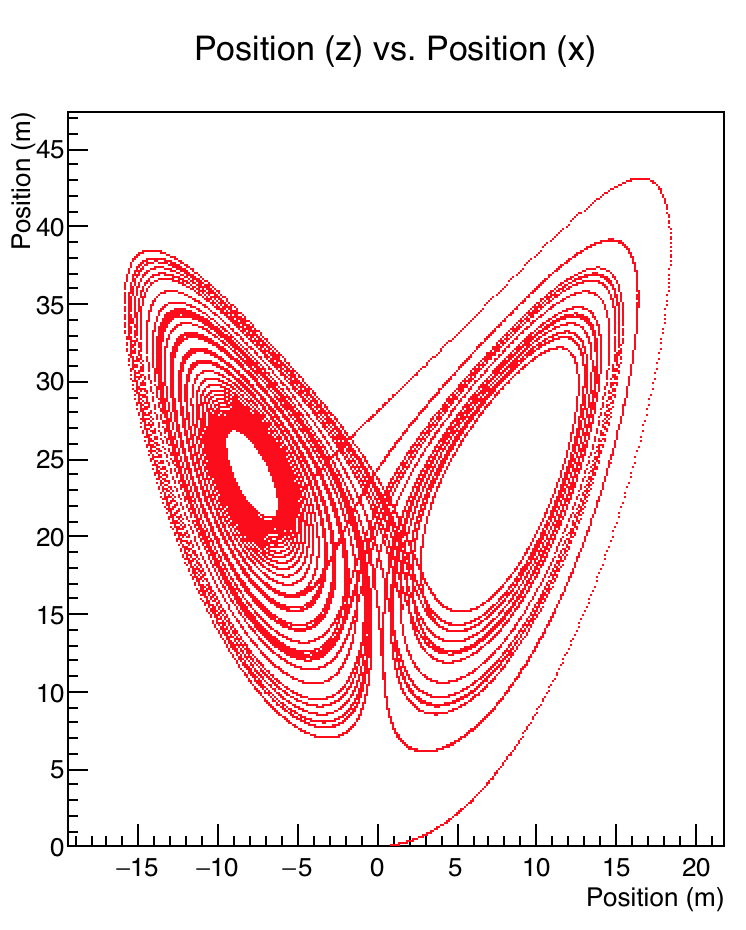
\includegraphics[scale=0.30]{fig-1.png}
			\caption{The Lorenz attractor, seen here as the $x$-$z$ projection of the solution.}
		\end{figure}
	\end{columns}
}

\frame{
	\frametitle{Results (continued)}
	
		\begin{columns}
		\column{0.4\textwidth}
		\begin{figure}[h]
			\centering
			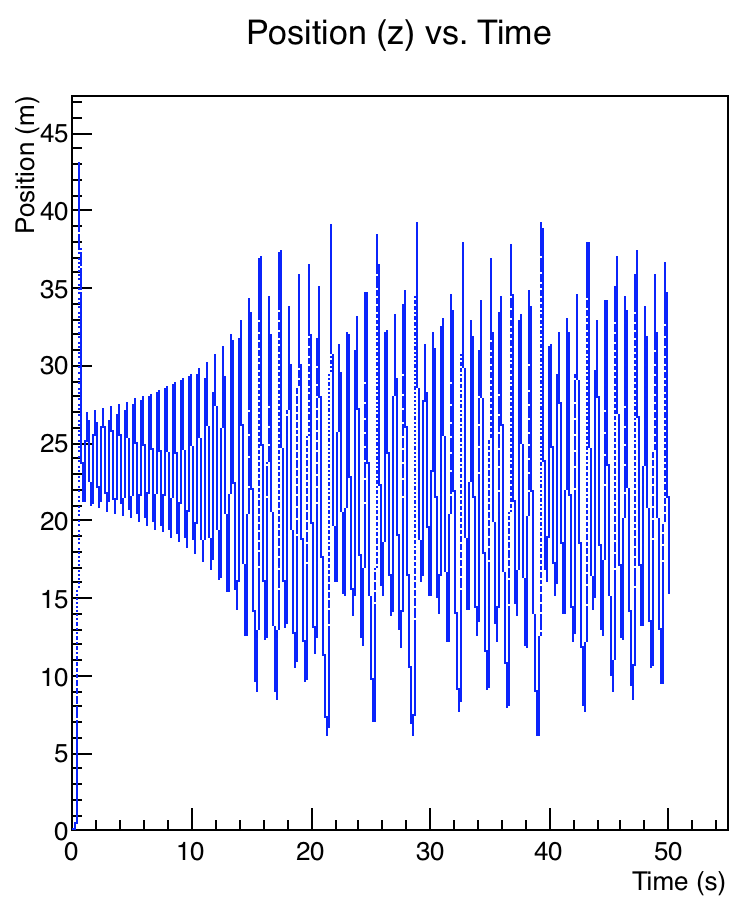
\includegraphics[scale=0.30]{fig-2.png}
			\caption{$z$ vs. $t$ after solving by the Euler method.}
		\end{figure}
		\column{0.6\textwidth}
		\begin{itemize}
			\item{Overall, was able to produce many of the graphics from the textbook, my graphs seemed visually accurate. }
			\item{ Found that the Lorenz model shows sensitivity to initial conditions. }
		\end{itemize}
	\end{columns}
}

\frame{
	\frametitle{Results (demo)}
	
	\begin{itemize}
		\item{The six graphs produced in my first program illustrate the overall behavior of the system. }
		\item{The second program demonstrates the system's sensitivity to initial conditions.  }
	\end{itemize}
	\begin{figure}[h]
			\centering
			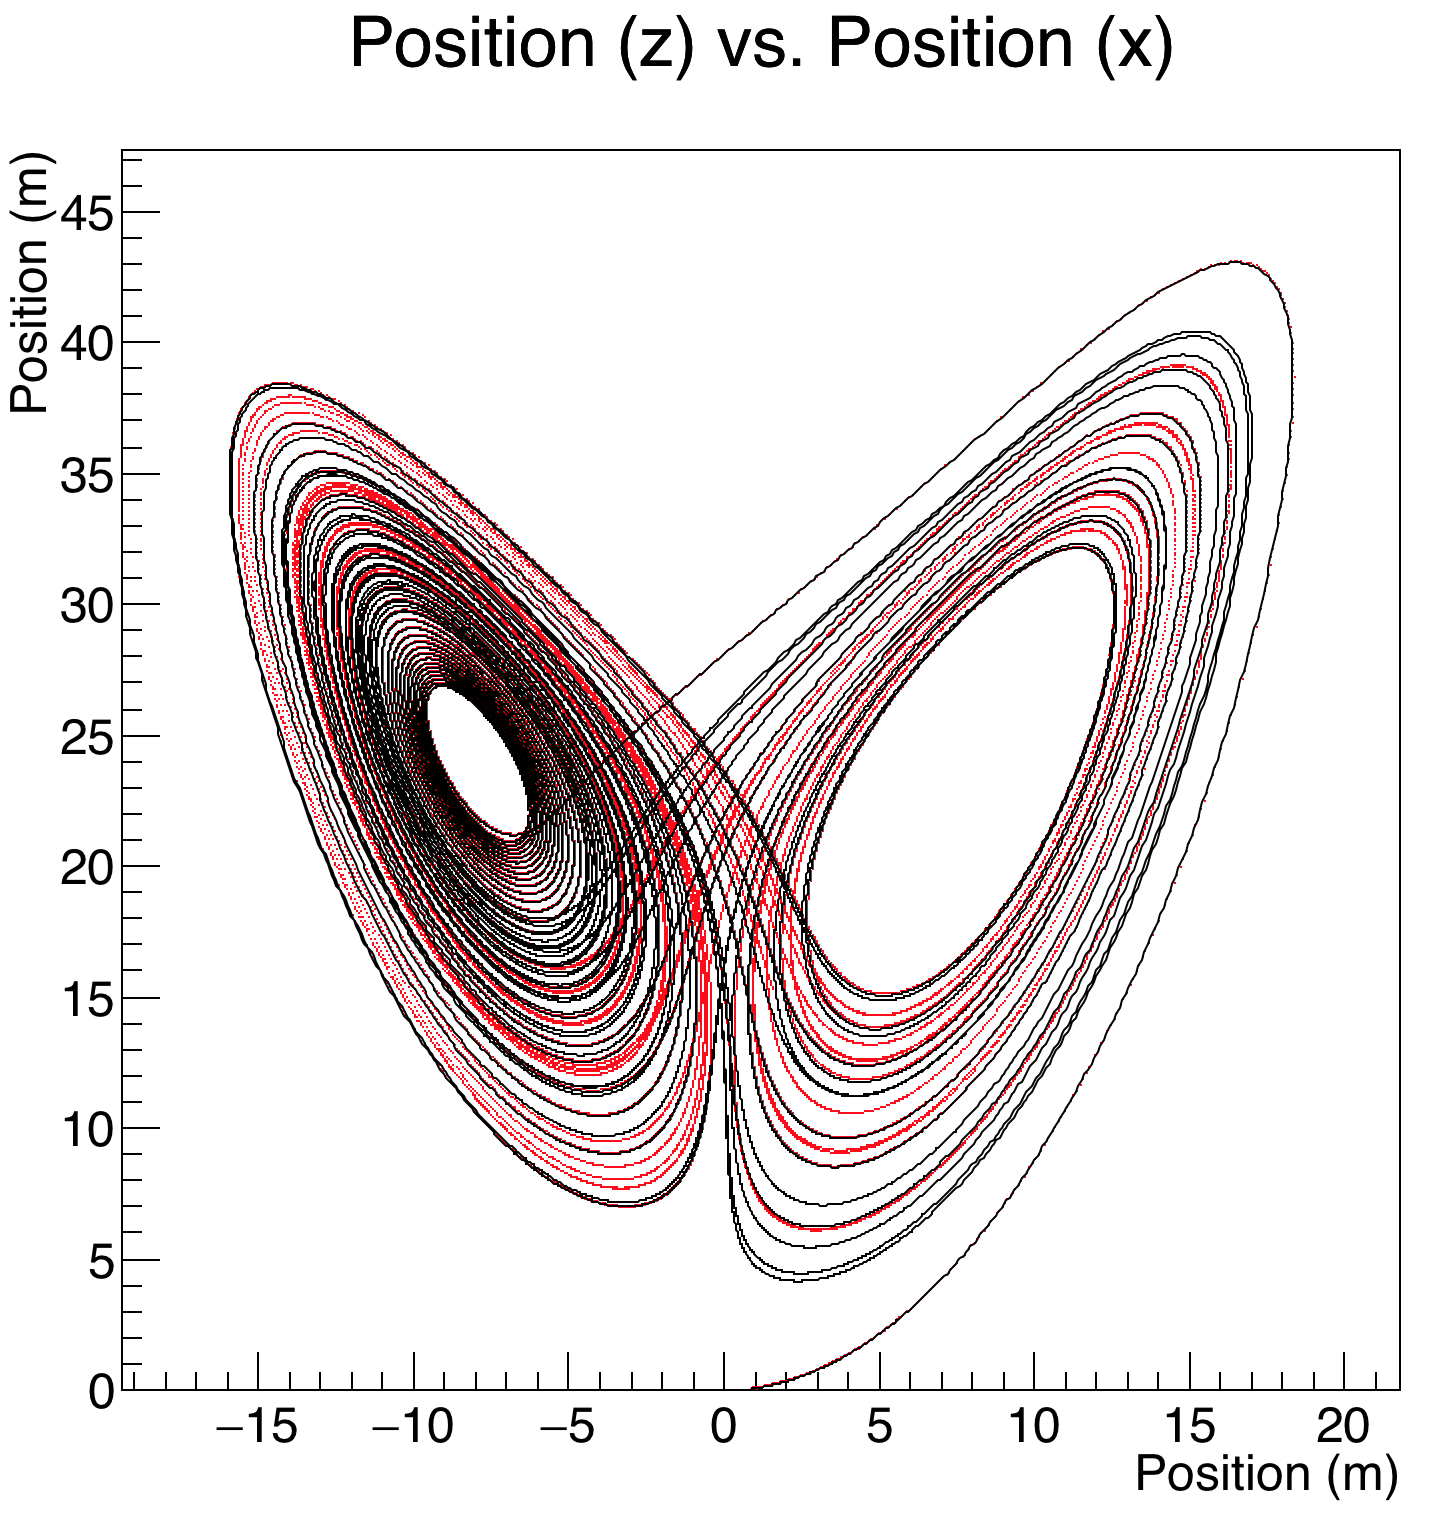
\includegraphics[scale=0.175]{fig-3.png}
			\caption{A sample output from my second program.}
	\end{figure}
}

\frame{
	\frametitle{Stability of the Numerical Method}
	
	\begin{columns}
		\column{0.6\textwidth}
		\begin{itemize}
			\item{Ran the program with $\Delta t = 2.0$, $1.0$, $0.1$, $0.01$, $0.001,$ and $0.0001$, but it failed for all $\Delta t \geq 0.01$,
			crashing while graphing due to $NaN$ values. }
			\item{At the high precisions required by the numerical method, more points are required. These can quickly exceed the
			limits of the $int$ type in C++, let alone the maximum array size.}
		\end{itemize}
		\column{0.4\textwidth}
		\begin{figure}[h]
			\centering
			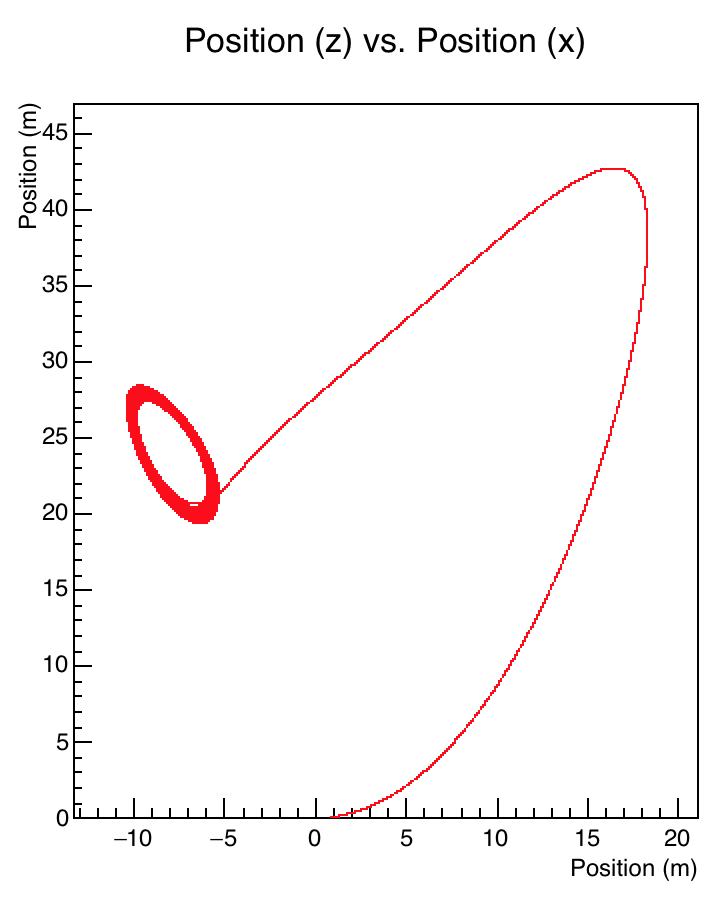
\includegraphics[scale=0.30]{fig-4.png}
			\caption{Not enough points to exhibit chaos: what about adding more points?}
		\end{figure}
	\end{columns}
}

\frame{
	\frametitle{Stability of the Numerical Method (continued)}
	
	\begin{itemize}
		\item{Altering the initial conditions and parameter values ends up having little impact on the correctness and accuracy of the Euler method.}
		\item{Increasing the parameters, particularly $b$, intensified the graphic. Acted almost like a measure of ``speed."}
		\item{Did not experiment with negative values of the parameters $\sigma$, $r$, and $b$ since they are positive by definition.}
	\end{itemize}
}

\frame{
	\begin{center}
		\blue{Questions?}
	\end{center}
}

\end{document}
